\documentclass{article}
\usepackage[english]{babel}
\usepackage[utf8]{inputenc}
\usepackage{fancyhdr}
\usepackage{geometry}
\usepackage{enumitem}
\usepackage{amsmath}
\usepackage{graphicx}
\usepackage[thinc]{esdiff}
\usepackage{tcolorbox}


\geometry{letterpaper, portrait, margin=1in}
\graphicspath{ {images/} }
\pagestyle{fancy}
\fancyhf{}
\lhead{Keerthik Muruganandam}
\rhead{Written Work 10}


\begin{document}

\begin{enumerate}[label=\textbf{(10.\arabic*)}]


\item How fast is the distance from an ant to the origin changing at the point $(4,2)$, if the ant moves along the line $y=\sqrt{x}$ and the $x$ coordinate increases at a rate of $3$ cm/s.
\newline
\newline
%START OF SOLUTION
We can find the rate of change for the distance from the origin if we find the derivative of the hypotenuse of the triangle formed from the points $(0,0)$, $(4,0)$, and $(4,2)$.
%FIGURE
\begin{figure}[h]
\centering
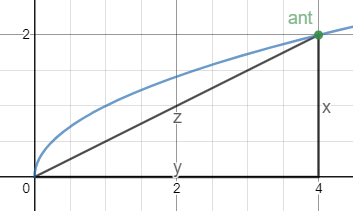
\includegraphics[scale=.5]{graph2}
\end{figure}
%END FIGURE
\newline
%DIFFERENTIATION
 We can use implicit differentiation of the Pythagorean Theorem to find $z^{\prime}$.
\[2xx^\prime+2yy^\prime=2zz^\prime\]
%SOLVE FOR VARIABLES
Now we need to find $y^\prime$ and $z$.
Use implicit differentiation on the function $y=\sqrt{x}$ to get
\[y^{\prime}=\frac{1}{2\sqrt{x}}x^{\prime}\text{.}\]
Now if we substitute x and y or 4 and 2 respectively and 3 for $x^{\prime}$, we get the equation
\[y^{\prime}=\frac{1}{2\cdot\sqrt{4}}\cdot 3 \text{.}\]
If we simplify the right hand side, $y^{\prime}$ equals $\dfrac{3}{4}$. The next step is to use the Pythagorean Theorem to find $z$.
\[4^2+2^2=z^2=\]
\[\sqrt{20}\]
%SUBSTITUTE/SOLVE
Now we substitute everything into $2xx^\prime+2yy^\prime=2zz^\prime$.
\[2\cdot4(3)+2\cdot2(\frac{3}{4})=2\sqrt{20}\cdot z^\prime\]
\[z^\prime=\frac{27}{4\sqrt{5}}\]
%END STATEMENT
The distance from the ant to the origin is changing at a rate of $\dfrac{27}{4\sqrt{5}}$ centimeters per second at this moment.
\newline

%NEW PROBLEM

\item A snowball melts at a rate equal to twice to its surface area. Find $\diff{r}{t}$ then record what you notice. 
%START OF SOLUTION (
The rate of melting is
\[\diff{V}{t}=2(4\pi r^2)\text{.}\]
To solve for $\diff{r}{t}$ we can differentiate the volume formula.
\[\diff{ }{t}(V=\frac{4}{3}\pi r^3)\]
\[\implies\diff{V}{t}=\frac{4\pi}{3}\cdot3r^2r^\prime=4\pi r^2r^\prime\]
If we substitute $\diff{V}{t}$ with $8\pi r^2$, we get the equation
\[8\pi r^2=4\pi r^2r^\prime\text{.}\]
Eliminating like terms and inserting a negative because the volume is decreasing yields the equation
\[\diff{r}{t}=2\text{.}\]
From this we can see that the rate of melting is constant.
\newline

%NEW PROBLEM

\item A conical water tank of radius 300 cm and height 500 cm leaks at a rate of 13 cm$^3$/min.The tank is being filled at a rate of 3 cm$^3$/min. Find the rate of change in water level when it is a 200 cm. \\
\newline
%START OF SOLUTION
We can construct two similar right triangles from the cross section of the water tank, one with the radius and height as sides, and the other with the water level and the corresponding width for sides.
%FIGURE
\begin{figure}[h]
\centering
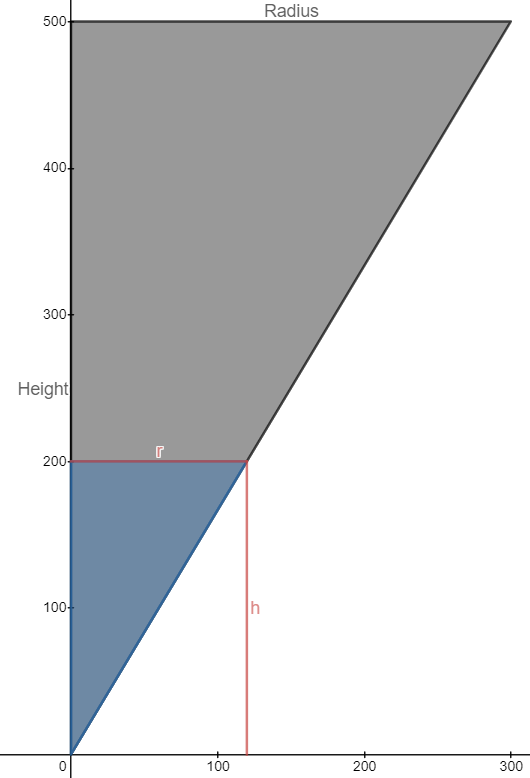
\includegraphics[scale=.25]{graph4}
\end{figure}
\par
Using the triangles with $r$ and $h$ defined as the radius and the height of the smaller triangle respectively, the relationship
\[\frac{300}{500}=\frac{r}{h}\]
can be found. Solving this gives the equation $r=\dfrac{3h}{5}$. Now we can substitute this into the equation for volume to get
\[V=\frac{1}{3}\pi {(\frac{3h}{5})}^2 h\text{.}\]
Simplifying gives us
\[V=\frac{3\pi}{25}h^3\text{.}\]
The next step is to use implicit differentiation on this equation and isolate $h^\prime$.
\[\diff{V}{t}=\frac{3\pi}{25}(3h^2h^\prime)\]
\[\implies h^\prime=\frac{25V^\prime}{9\pi h^2}\]
Now substitute $V^\prime$ for -10 cm$^3$/min and $h$ for 200 cm. $V^\prime$ is negative because the tank is being emptied faster than being filled.
\[h^\prime=\frac{25(-10)}{9\pi(200)}=\frac{-250}{1800\pi}=-\frac{5}{36\pi}\]
The water level is changing at a rate of $-\dfrac{5}{36\pi}$ cm$^3$/min.
\newpage

%NEW PROBLEM

\item \textbf{Professional Problem:} A batter hits the ball and runs toward first base with a speed of $f(t)$  after $t$ seconds. If it takes the batter 2 seconds to reach halfway to to first base, at what rate is the distance to second base decreasing at this time.

First, a diagram of the scenario should be drawn. From an aerial view, the pitch looks like this:
\begin{figure}[h]
\centering
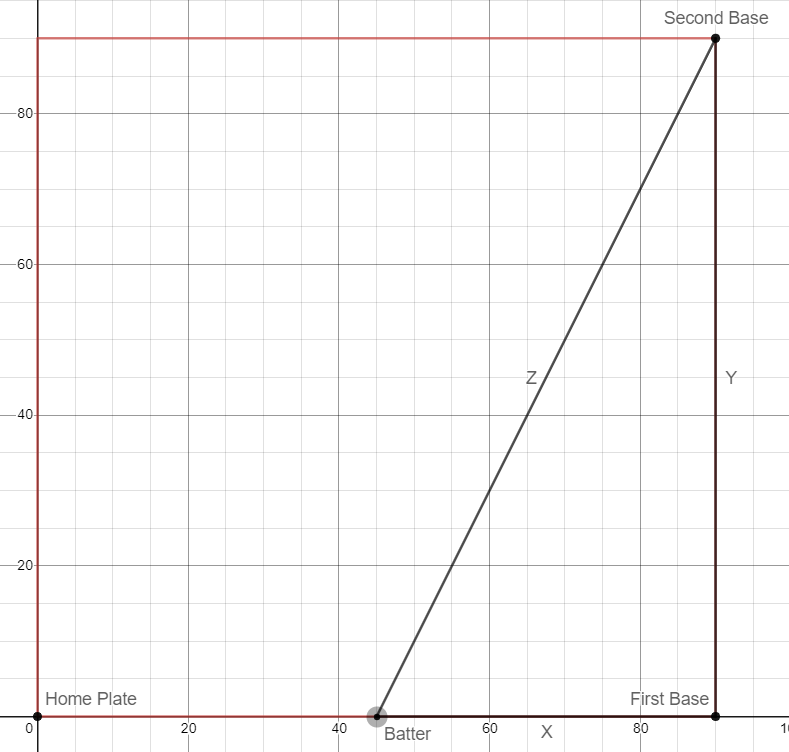
\includegraphics[scale=.30]{graph3}
\end{figure}
\par
We want to find $\diff{Z}{t}$ because we need to find the speed the distance between the batter and second base is changing. We can use the Pythagorean Theorem in this scenario to find $Z^\prime$ because of the triangle shape. The differentiated version of the Pythagorean Theorem looks like
\[2ZZ^\prime=2XX^\prime\text{.}\]
Since the distance from first base to second base is constant, $Y$ was canceled out. After isolating $Z^\prime$, the equation looks like
\[\frac{XX^\prime}{Z}=Z^\prime\text{.}\]
Now we need to calculate values for $Z$, $X^\prime$, and $X$. $X^\prime$ is equal to $-f(t)$ because $X$ decreasing and since $f(t)=22.5$, $X^\prime=-22.5$ ft/sec. X can be defined as ($90-f(2)$) because the length of $X$ is how much has not been covered by $f(t)$ of 90. Therefore, $X=45$ ft. To find $Z$ use the Pythagorean Formula like so
\[\sqrt{45^2+90^2}=\sqrt{10125}=15\sqrt{5}\text{ ft.}\]
Now we substitute in our values to produce to expression
\[\frac{-22.5(45)}{15\sqrt5}\text{.}\]
Simplifying produces the final number of
\[-\frac{2025}{30\sqrt{5}}\text{.}\]
\par
Before providing the final answer, $-\dfrac{2025}{30\sqrt{5}}$ must be multiplied by $-1$ because the question asks for the rate when it is \textit{decreasing} and the rate was found without consideration of direction. The reasoning is when the reader doesn't know the direction, the negative sign will show that the value is decreasing. However, because the question asks for the rate when decreasing, the negative sign is redundant or could even be interpreted as $X$ is increasing. Thus
\[Z^\prime=-1\cdot-\frac{2025}{30\sqrt{15}}=\frac{2025}{30\sqrt{15}}\text{.}\]
\par
\begin{tcolorbox}[colback=white]
\center
The batter's distance to second base is decreasing at a rate of $\frac{2025}{30\sqrt{15}}$ ft/sec.
\end{tcolorbox}

\end{enumerate} 

\end{document}

